\section{Findings}
\label{sec:findings}

\begin{table}[htbp]
\scriptsize
\setlength{\tabcolsep}{3pt}
\renewcommand{\arraystretch}{1.1}
\begin{tabularx}{\linewidth}{
  >{\hsize=0.7\hsize}X
  >{\hsize=0.7\hsize}X
  >{\hsize=0.9\hsize}X
  >{\hsize=0.9\hsize}X
  >{\hsize=0.9\hsize}X
  >{\hsize=0.9\hsize}X
  >{\hsize=0.9\hsize}X
  >{\hsize=0.5\hsize}X
  >{\hsize=0.6\hsize}X
}
\toprule
\textbf{pearson\_r} & \textbf{pearson\_p} & \textbf{mae} & \textbf{rmse} &
\textbf{mape\_\%} & \textbf{ba\_diff\_mean} & \textbf{ba\_diff\_sd} &
\textbf{domain} & \textbf{region}\\
\midrule
0.0216483 & 0.6291557 & 9.7345e15 & 8.71e16 & 8.66e9 & -9.7345e15 & 8.6642e16 &
core & ALL\\
-0.0137426 & 0.7591933 & 2.8836e16 & 1.4556e17 & 4.03e9 & -2.8836e16 & 1.4282e17 &
package & ALL\\
0.0173603 & 0.8638830 & 1.0789e15 & 6.7850e15 & 2.36e9 & -1.0789e15 & 6.7324e15 &
core & burst\_10s\\
-0.0244561 & 0.8091504 & 3.8958e13 & 2.3453e14 & 1.51e7 & -3.8958e13 & 2.3243e14 &
core & burst\_60s\\
-0.0572145 & 0.5717915 & 1.3919e5 & 2.3117e5 & 1.66e2 & 2.2276e4 & 2.3126e5 &
core & idle\_10s\\
0.0186232 & 0.8540869 & 3.2491e16 & 1.6279e17 & 3.76e10 & -3.2491e16 & 1.6032e17 &
core & static\_10s\\
0.0860196 & 0.3947917 & 1.5064e16 & 1.0671e17 & 3.30e9 & -1.5064e16 & 1.0617e17 &
core & static\_60s\\
-0.0696231 & 0.4912554 & 4.4687e16 & 1.1565e17 & 9.78e9 & -4.4687e16 & 1.0721e17 &
package & burst\_10s\\
0.0146812 & 0.8847316 & 2.5601e16 & 8.5340e16 & 9.93e8 & -2.5601e16 & 8.1820e16 &
package & burst\_60s\\
0.0101416 & 0.9202304 & 2.7044e15 & 2.7044e16 & 1.84e9 & -2.7044e15 & 2.7044e16 &
package & idle\_10s\\
-0.1129127 & 0.2633483 & 4.8429e16 & 2.4218e17 & 6.93e9 & -4.8429e16 & 2.3849e17 &
package & static\_10s\\
0.1083681 & 0.2831723 & 2.2756e16 & 1.6091e17 & 5.89e8 & -2.2756e16 & 1.6010e17 &
package & static\_60s\\
\bottomrule
\end{tabularx}
\caption{Statistics.}
\label{tab:stats}
\end{table}

The analysis of metrics and plots revealed no evidence of dynamic agreement
between \texttt{ryzen\_smu} and \gls{RAPL} energy-measurement interfaces
across the investigated domains and workload regions.

Key observations are as follows:

\begin{itemize}
  \item \textbf{Correlation:} Pearson coefficients are close to
  zero in all cases (\(r \in [-0.11,0.11]\), \(p \gg 0.05\) (\cref{tab:stats})),
  indicating absence of linear correlation between readings for both \emph{core}
  and \emph{package} domains.

  \item \textbf{Error Metrics:} Absolute error metrics are large across
  all regions. \gls{MAE} and \gls{RMSE} frequently reach \(10^{16}\!-
  \!10^{17}\,\mu\mathrm{J}\) (\cref{tab:stats}), and \gls{MAPE} in most cases
  exceed several orders of magnitude, underscoring substantial differences in
  absolute energy values.

  \item \textbf{Bland–Altman Plots:} Mean differences are
  far from zero with very wide limits of agreement, highlighting a systematic
  bias and considerable dispersion between two measurement sources.
\end{itemize}

\begin{figure}[htbp]
    \centering
    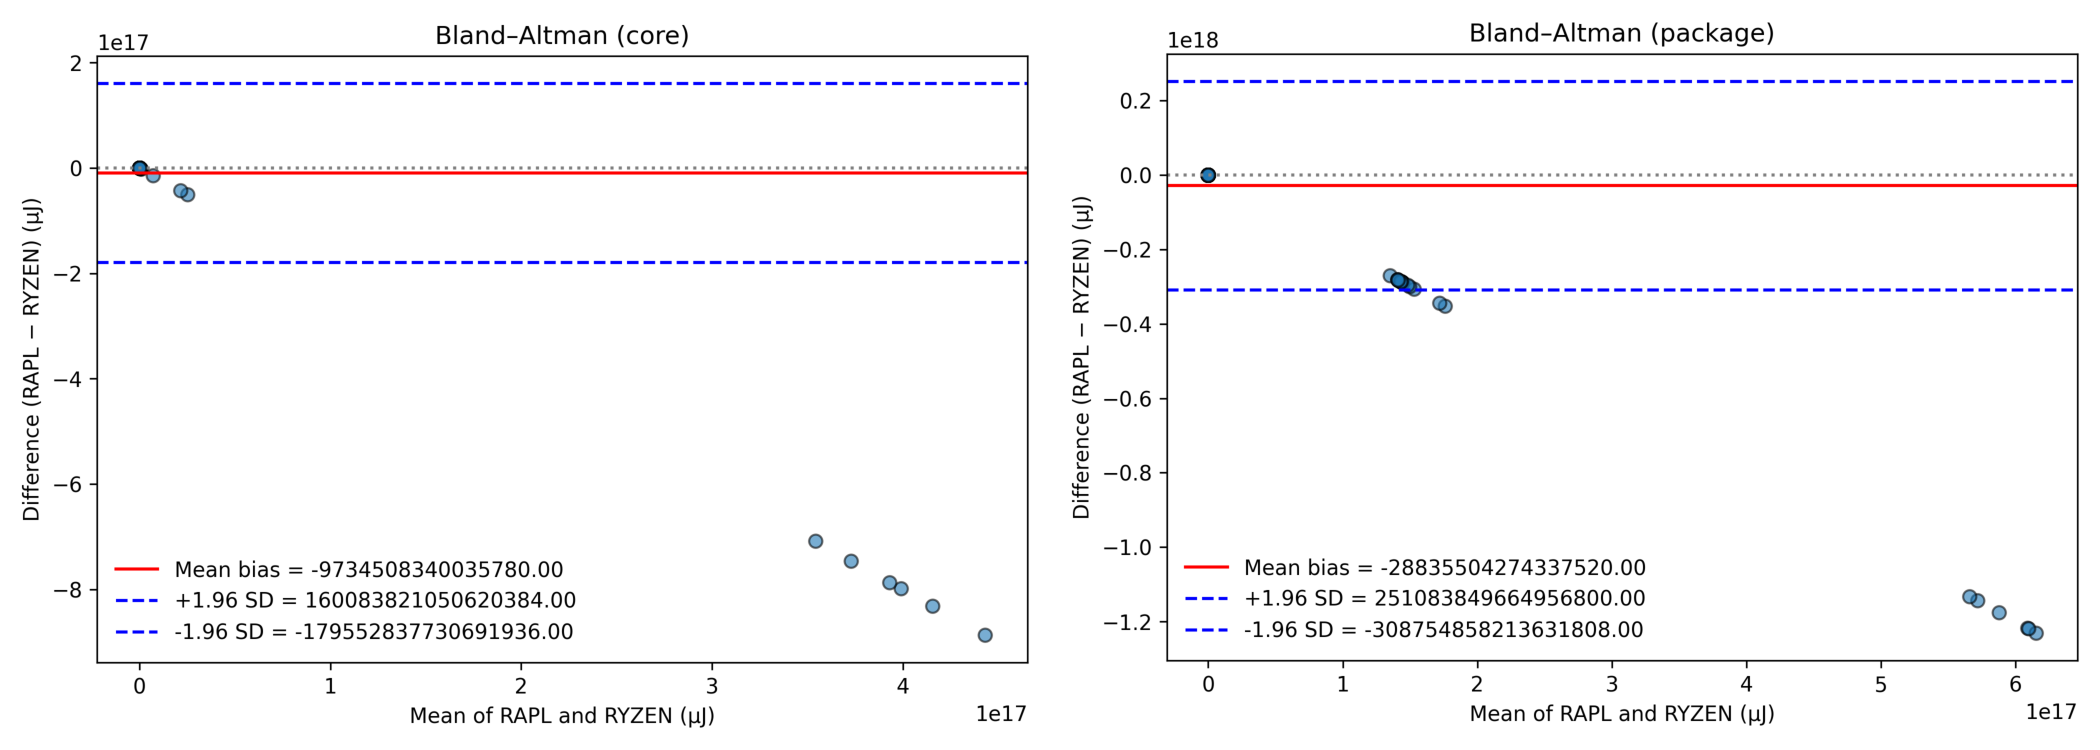
\includegraphics[width=0.9\textwidth]{assets/bland_altman}
    \caption{Main Bland-Altman Plots for \emph{core} and \emph{package} domains.}
    \label{fig:plots}
\end{figure}

Collected results contradict the initial expectation of high dynamic
correlation and practical interchangeability between \texttt{ryzen\_smu} and
\gls{RAPL} measurements, thus not allowing to disprove the $H_{0}$
(\cref{sec:hypo}).

Full Bland-Altman plots for all \emph{Measurement Regions} and \emph{Power Domains}
are available in Appendix \cref{app:plots}.

\subsection{Per-Core Measurements Potential}

It was identified during this research that \texttt{ryzen\_smu} kernel driver
allows to obtain per-core power readings of the \gls{CPU}. However,
observations of those readings gave a strong suspicion about their reliability
. As described in \cref{sec:limncons}, since the mappings of \gls{PM} table
were reverse engineered, it is highly possible that the values read from the
addresses are not the power readings, but rather some other unrelated
telemetry values.

The main source of concern is the fact that in all the test runs the third
and sixth cores consistently reported 0 power consumption. (Can be inspected
in the raw measurement outputs included in supporting repository
\footcite{yahdzhyiev2025repo}).

With that mentioned, the fact of the possibility to have per-core measurements
available highlights potential benefits of using \texttt{ryzen\_smu} for
energy readings in \gls{HPC} cluster environments where resource sharing is
supported (meaning two jobs/processes occupying different physical cores of 
the same \gls{CPU}).

\subsection{Sampling/polling Rate Experiments}
\label{sec:find:rates}

Despite the statement in \textcite{ryzen_managment_linux} that
\texttt{ryzen\_smu} driver intentionally limits the refresh rate to
approximately 1 milli-second small practical tests/experiments with
\texttt{monitor} (see \footcite{yahdzhyiev2025repo} \path{code/src/monitor.c})
and \texttt{profile} (see \footcite{yahdzhyiev2025repo}
\path{code/src/profile.c}) showed the possibility of obtaining distinct energy
readings from \gls{PM} Table on much higher rates (approx. 1 micro-second)
(as also mentioned in \cref{sec:limncons}).

The outputs of \texttt{sudo ./profile} with polling/sampling rate set to
1 micro-second can be inspected in \cref{app:outputs}.

Additional tests were carried out via \gls{EMA} (included) profiling utility
(which also was the author's contribution \footcite{
  Source code available at \url{
    https://github.com/SerhiiYahdzhyiev/EMA/tree/profiler/utils/profiler
  }
}), additionally proving higher sampling frequency capabilities of
\texttt{ryzen\_smu}. Raw outputs available in early mentioned supporting
repository and also in Appendix \cref{app:outputs} (raw outputs were truncated
for clarity and conciseness).

These results might be explained by the combination of the statements from the
same source \parencite{ryzen_managment_linux}:

\begin{itemize}
  \item The \gls{SMU} itself is sampling its internal sensors at a very high
    frequency, likely in the kilohertz (kHz) range, to make its own power
    management decisions.
    This is the ultimate physical limit, and it is not publicly documented.
  \item Here is a summary and explanation of the \texttt{ryzen\_monitor} and
    \texttt{ryzen\_smu} software projects, with a focus on the
    \emph{AMD Ryzen 5 5625U processor}.
\end{itemize}
 \parencite{ryzen_managment_linux}

As can be seen in the last statement the model and architecture of the target
\gls{CPU} for the contents of the source differs from the test system's (
see \cref{app:hwspec}), additionally the source does not specify which
\gls{BIOS} version was used to test/obtain basis for the statements provided.

The mentioned small tests/experiment can be used as a basis for a separate
research with extended methodology that should include external \gls{PMD}
as the source of truth to evaluate the reliability of the readings
obtained at increased sampling rates. They also can be a part of the
basis for extensions and improvements of the methodology used for this
research.
